% Resources 
\chapter{Recursos}

% Personnel 
\section{Pessoal}

% Size of staff for the project 
\subsection{Tamanho da equipe para o projeto }
Tamanho da equipe: 2 pessoas.

% Software 
\section{Software}


% Identify  software  needed  to  support  system  (includes  system  plus SEE/STE/tools requirements) 
\subsection{Identificar o software necess�rio para suportar o sistema}
O software necess�rio � um sistema operacional com navegador instalado, podendo ser Google Chrome acima da vers�o 59.0.3071, ou Firefox acima da vers�o 50.0

% Hardware 
\section{Hardware}
Requisitos do hardware.

% Identify hardware needed to support system (includes system plus SEE/STE requirements) 
\subsection{Identificar o hardware necess�rio para suportar o sistema}

% Facilities 
\section{Instala��es}

% Identify facilities requirements
\subsection{Identificar requisitos de instala��es}
Possuir internet.

% Special procedural requirements (e.g., security, access rights, and documentation control)
\section{Requisitos processuais especiais (por exemplo, seguran�a, direitos de acesso e documenta��o ao controle)}
N�o h�.

% Cost estimating 
\section{Estimativa de custo}

% Describe the cost estimating method 
\subsection{M�todo da estimativa de custo}
Pontos por caso de uso.

% Documentation 
\section{Documenta��o}

% Software Quality Plan
\subsection{Plano de qualidade do software(ISO 9126)}

As mudan�as ser�o nos �mbitos de confiabilidade e usabilidade.

\begin{description}
	\item[Confiabilidade] as corre��es visam corrigir falhas no software.
	\item[Usabilidade] as mudan�as visam melhorar o visual do site para torn�-lo mais atrativo ao usu�rio.
\end{description}

% Project Management Plan 
\subsection{Plano de Gerenciamento de Projeto}

\begin{figure}[!hb]
	\centering
	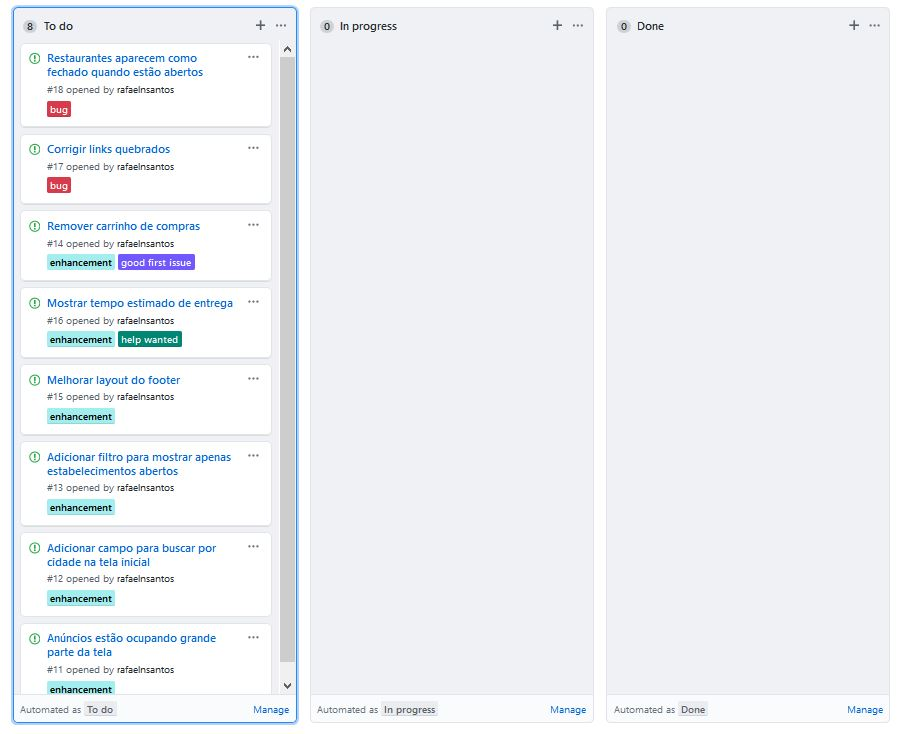
\includegraphics[width=\linewidth]{images/kanban.jpg}
	\caption{}
	\label{fig:kanban}
\end{figure}

% Configuration Management Plan
\subsection{Plano de Gerenciamento de Configura��o}

% Measurement Plan
\subsection{Plano de Medi��o}

% Development documents
\subsection{Documentos de desenvolvimento}

\pagebreak

% Maintenance manuals
\subsection{Manuais de manuten��o}
\begin{figure}[!hb]
	\centering
	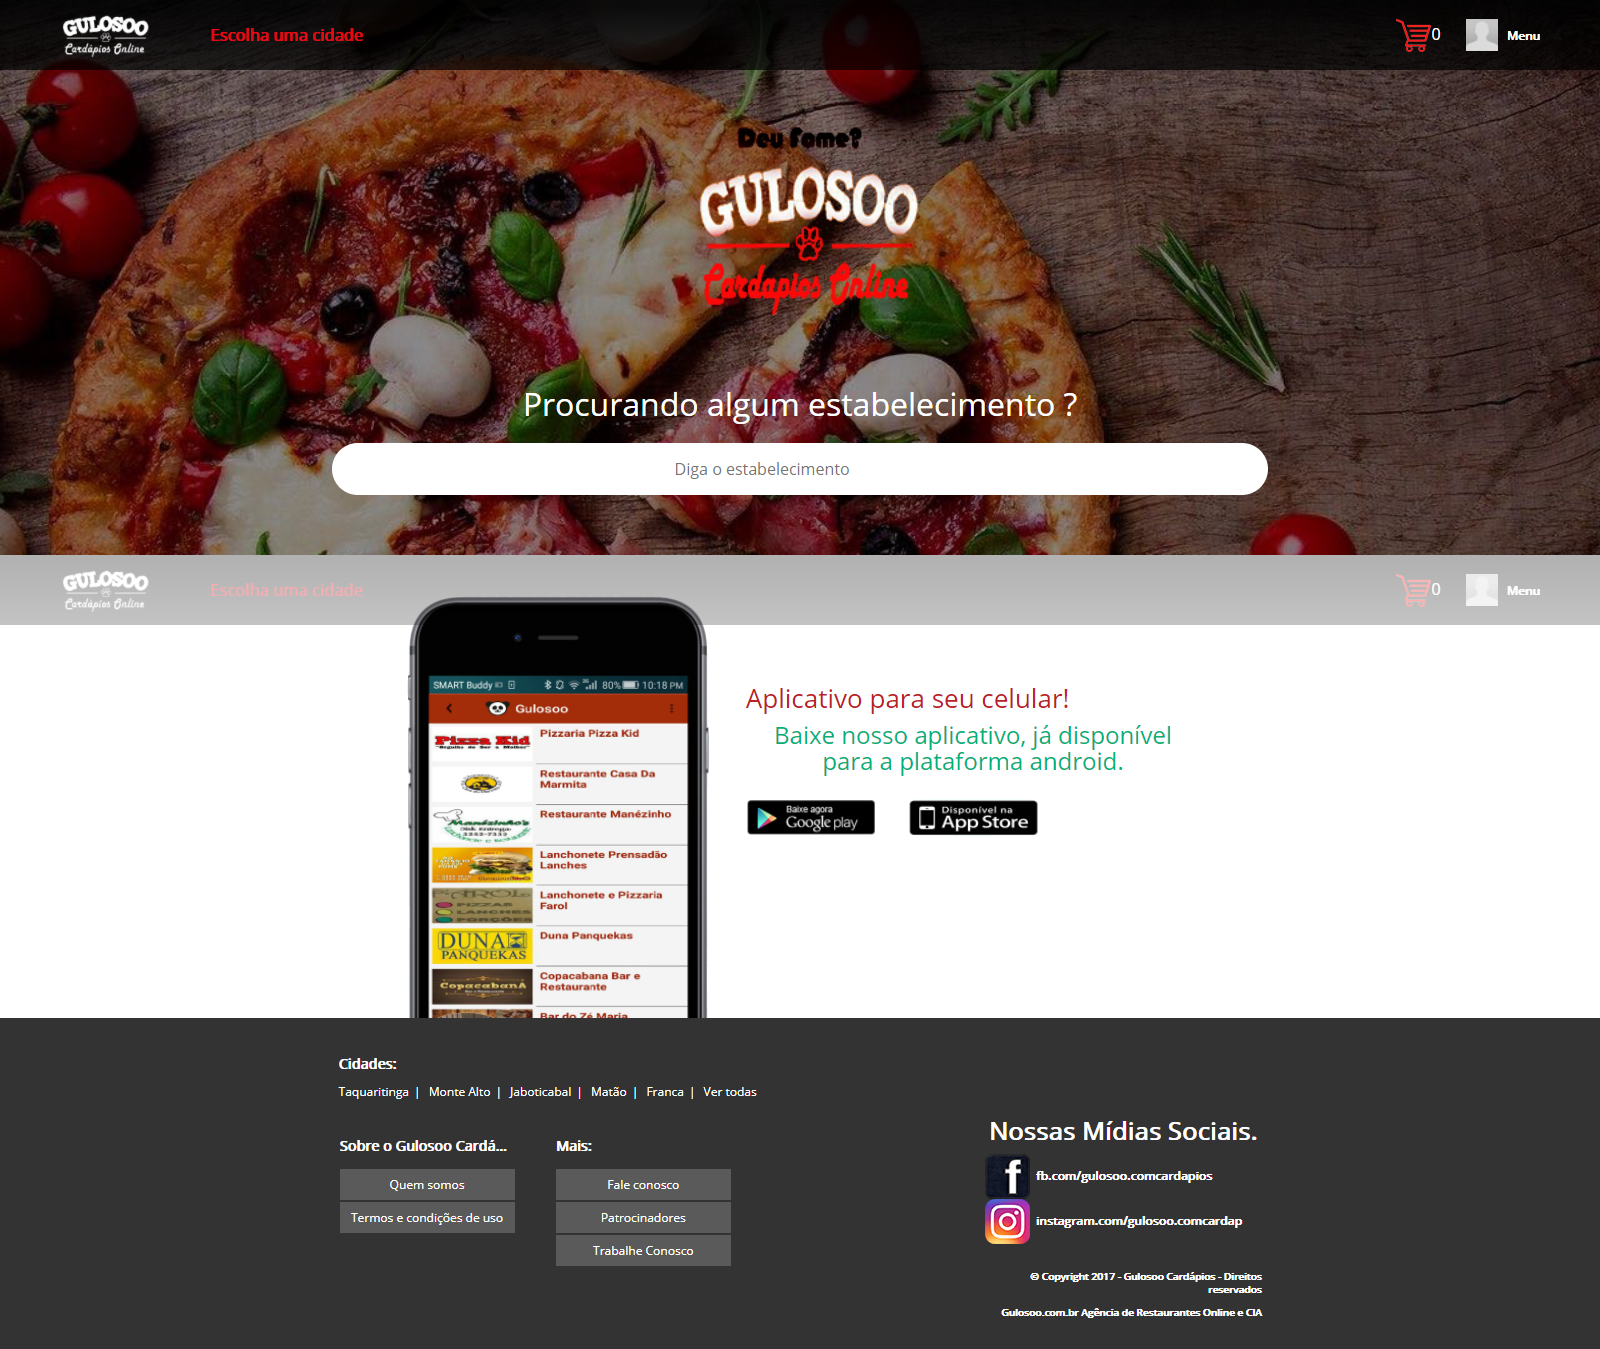
\includegraphics[width=\linewidth]{images/home.png}
	\caption{}
	\label{fig:home}
\end{figure}

\pagebreak

\begin{figure}[!hb]
	\centering
	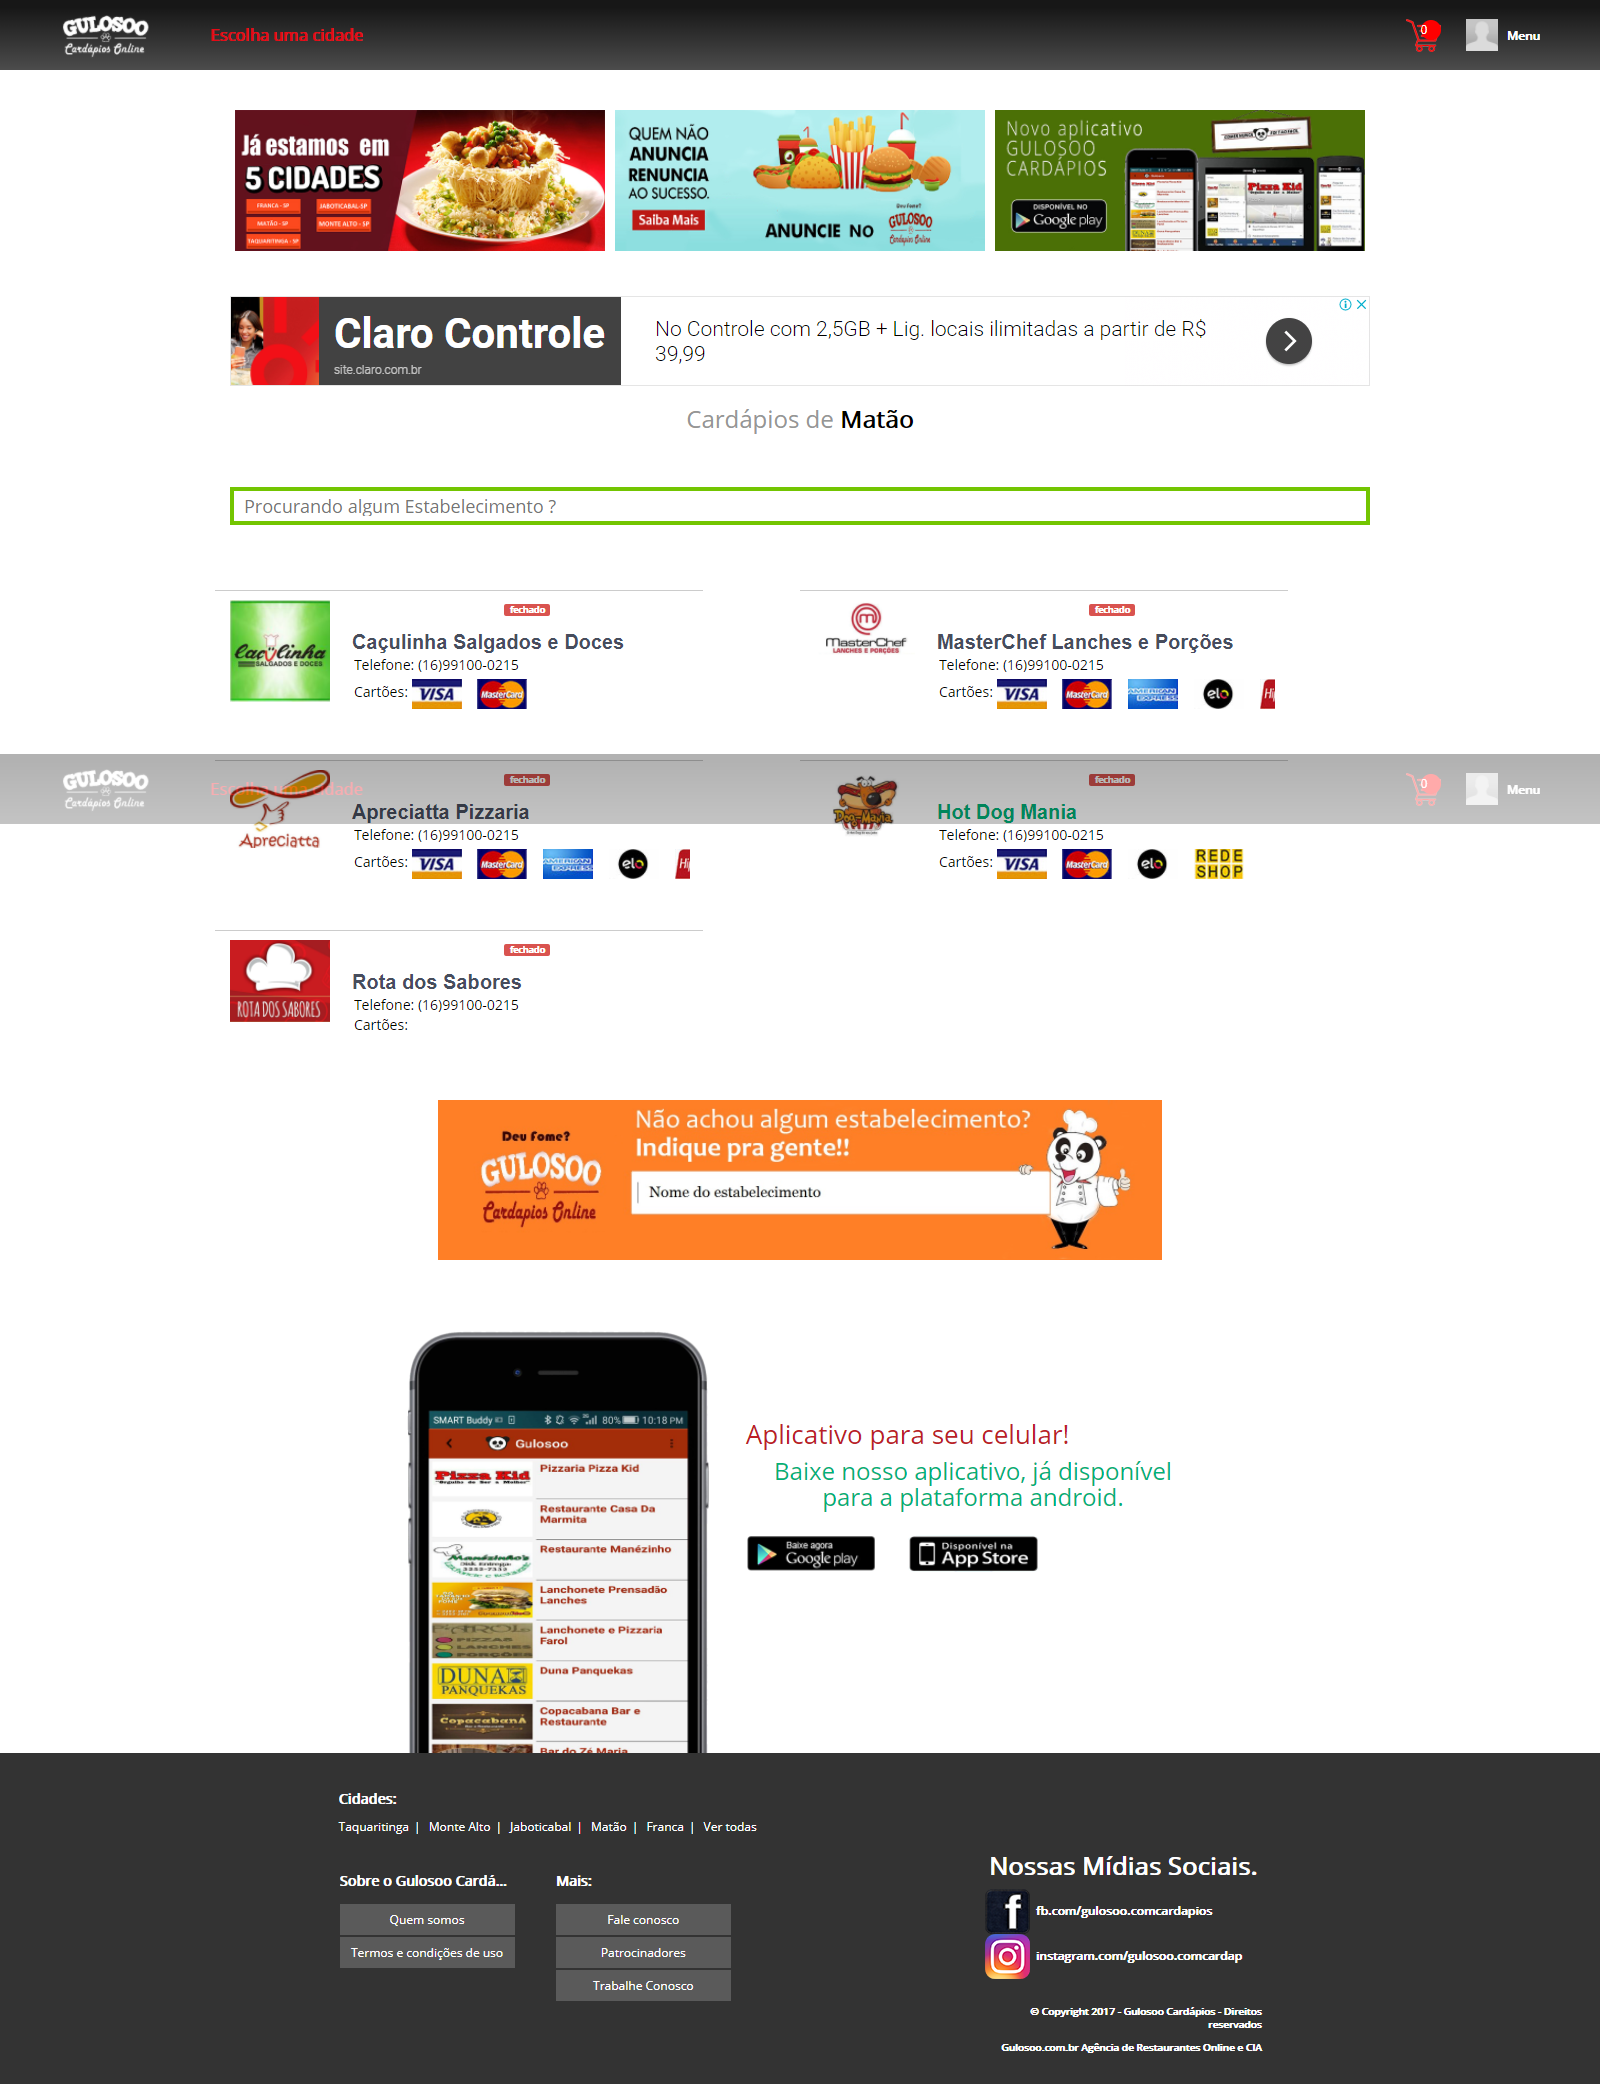
\includegraphics[width=\linewidth]{images/estabelecimentos.png}
	\caption{}
	\label{fig:estabelecimentos}
\end{figure}

\pagebreak

\begin{figure}[!hb]
\centering

\includegraphics[width=\linewidth]{images/cardapio.png}
\caption{}
\label{fig:cardapio}
\end{figure}

\pagebreak

% Verification Plan
\subsection{Plano de Verifica��o}

% Validation Plan
\subsection{Plano de valida��o}

% Test Plan, Test Procedures, and Test Reports
\subsection{Plano de teste, procedimentos de teste e relat�rios de teste}

% Training Plan 
\subsection{Plano de Treinamento}
O treinamento ser� realizado atrav�s de programa��o em par.

% User?s Manual(s)
\subsection{Manual(s) do Usu�rio}
N�o se aplica.

% Data management
\section{Gerenciamento de dados}
Github.

% Identify repositories 
\subsection{Reposit�rios}

% Other resource requirements (if needed)
\section{Outros requisitos de recursos (se necess�rio)}
N�o se aplica.
